\acresetall
\chapter{Conclusions}
\label{ch:conclusions}

\section{Summary}
In the preceding chapters I have laid out an understanding of memory in general, but also more specifically spatial-episodic memory, the structure in the brain that supports it (the hippocampus) and place cells as the functional units of these memories (\autoref{ch:intro:memory}).
I have explained the symptoms that define \scz/, particularly the cognitive deficits which are most relevant for functional recovery, yet least treatable, and identified some of the underlying genetic risk factors and proximate causes (\autoref{ch:intro:scz}).
I described the techniques that I employed inf my experiments as well and the tools I developed to run the experiments and analyze the data (\autoref{ch:intro:techniques}).
I next presented my primary thesis work; the characterization of hippocampal area CA1 pyramidal cell functional alterations during spatial learning in the \df/ mouse model of \scz/ (\autoref{ch:df}).
In addition, in collaboration I developed a Python package for the initial processing of Ca\super{2+} imaging data that we have released to the broader neuroscience community (\autoref{ch:sima}).
Supplementing my primary project, I also help characterize the \emph{in vivo} functional properties of long-range inhibitory projections from lateral entorhinal cortex to CA1, adult-born granule cells among the dentate gyrus granule cell population, and developmentally separable sub-populations of pyramidal cells within CA1 (\autoref{ch:other}).

It's worth noting that that while my main paper primarily looked to understand aberrant hippocampal activity in the \df/ mouse during spatial-reward learning task, my data also is interesting from the reverse perspective of understanding normal hippocampal function during a spatial-reward learning task.
We have shown that the \df/ mouse is a model of impaired global remapping (context stability) and goal-related remapping (enrichment), two fairly complicated properties of neuronal circuits that would otherwise be very difficult, if not impossible, to manipulate.
From this perspective, my data provides evidence that inducing global remapping or preventing reward-zone place cell enrichment impairs spatial-reward memory.

% \subsection{What we learned about memory}

% It's impossible to talk about declarative memory without quickly getting to discussions of the \ac{HPC}.
% By performing some of the first functional \emph{in vivo} imaging experiments in the \ac{HPC} I characterized the \emph{in vivo} activity of novel circuit elements and showed how this activity mapped on to behavior.



% \subsection{What we learned about \scz/}

% Minor changes to context resulted in global remapping in \df/ mice, lending support to the idea of \scz/ as a disorder of aberrant salience.

\section{Future directions}

% There remains several open questions directly related to my work as well as new related areas of research.

% follow-up experiments 
% new experiments
% new compartments
% new mice

\subsection{Context generalization}
My \ac{GOL} task tested two fundamentally different aspects of spatial memory: How do spatial maps change in response to small changes to the environment (Condition~I \& II)? and How do spatial maps support the encoding of salient reward locations (Condition~II \& III)?
I found an interesting differential effect between WT and \df/ mice in both of these tasks, so it would be interesting to explore each of these in more detail.
In particular, my context remapping results suggests that the \df/ mis-attend to stimuli that the wildtype mice ignore, which manifests as an over-separation of similar contexts as seen by impaired task performance and also the global remapping of spatial maps between the two similar contexts.
This could be looked at in more detail by systematically modifying the two contexts to have varying degrees of symmetry and look at similarity of spatial maps between the two contexts while performing a context discrimination task.

\subsection{Interneurons}
Hippocampal area CA1 consists not only of a dense pyramidal cell layer, but also diverse populations of local GABAergic interneurons which control pyramidal cell spiking \citep{Freund1996}.
Two main classes of pyramidal cell-targeting GABAergic neurons -- dendrite-targeting (e.g. somatostatin-positive; SST+) and soma-targeting (e.g. parvalbumin-positive: PV+) interneurons -- have been shown to directly modulate pyramidal cell burst spiking and theta phase repsectively \citep{Royer2012}\citep{Lovett-Barron2012}.
A third potentially interesting classification of interneurons in the \ac{HPC} are the interneuron-targeting vasointestinal peptide expressing (VIP+) interneurons, which are less well understood, but can drive \ac{HPC} pyramidal cell activity though disynaptic disinhibition \citep{Chamberland2012}.
\todo[color=yellow]{Expand on VIP cells}
Importantly, an excitatory-inhibitory imbalance has also been implicated as a possible root cause of \scz/ progression (see \autoref{sec:intro:scz:glutamate}).
Goal oriented learning-related reorganization of hippocampal CA1 interneuron activity has been recently demonstrated \citep{Dupret2013}, suggesting that CA1 GABAergic interneuron activity is closely tied to learning-related remapping of place cell ensembles, but the role of genetically-identified \ac{HPC} GABAergic inhibitory circuits during normal and diseased learning and memory has not been characterized.
In particular, the paper by \citeauthor{Dupret2013} shows that interneuron activity evolves with pyramidal cell activity as learning progresses and place cells enrich the reward location.
It is tempting to infer that interneuron activity is shaping pyramidal cell activity profiles, as it is possible that local interneurons could provide the needed signal to shift place cell firing towards the reward location.
By recording the activity of dendrite-targeting and soma-targeting interneurons during the \ac{GOL} task I can look for altered activity during Condition~III, when the \df/ mice failed to show any reward enrichment, and also performed poorly on the task.
\todo[color=yellow, inline]{Include mention of prelim VIP data?}

\subsection{Imaging during alternate hippocampus-dependent behaviors in \df/ mouse}
Goal-oriented learning, as a test of spatial-episodic memory, was the first behavior -- beyond simple random-foraging tasks -- that we attempted to train the head-fixed \df/ mice to perform.
It would also be very interesting to analyze behaviors related to other cognitive domains with well-known deficits in the \df/ mice.
The \df/ mice have a well-established deficit in contextual fear conditioning \citep[CFC,][]{Stark2008} -- they freeze less than wildtype mice -- and we have already adapted CFC for head-fixed imaging \citep[hfCFC,][]{Lovett-Barron2014}.
Our hfCFC uses an airpuff to the snout, instead of a foot shock, as the unconditioned stimulus (US) and lick suppression, instead of freezing, as the conditioned response (CR), so we would need to confirm that the \df/ still showed a behavioral deficit with this potentially milder US.
Based on the work by \citeauthor{Moita2004}, I would expect to see place cell remapping selectively induced in the wildtype mice in the conditioned context, but not in the \df/ mice.
In addition, we have shown that SST+ interneurons in CA1 effectively filter out the CS from the representation of the conditioned context \citep{Lovett-Barron2014}, so disrupted interneuron activity in the \df/ mice could lead to contamination of the conditioned context representation in the \ac{HPC} by the US, leading to the observed deficit in freezing.
This would also be generally consistent with my finding that the \df/ mice are differentially affected by small changes to the contextual environment (\autoref{sec:df:results:context}) and the \scz/ conceptual framework that suggests that mis-attribution of salience may be the the fundamental underlying dysfunction \citep{Kapur2003a}\citep{VanOs2009}.

Another interesting behavior for future study is prepulse inhibition (PPI), where the magnitude of the acoustic startle response to a loud noise is markedly reduced by preceding the tone with a milder stimulus.
The \df/ mouse shows decreased PPI, and this behavior involves the septo-hippocampal cholinergic projection in particular \citep{Koch1996}\citep{Swerdlow2001}.
This task should be fairly straightforward to establish as a head-fixed paradigm.
As place cells and running activity would not necessarily be relevant for this task, I could instead use an immobilization chamber in place of the treadmill that I used throughout my previous experiment.
Mice quickly adapt to this form of restraint and other members of our lab regular make use of this technique.
The aversive stimulus could be either an airpuff as we've used in the past, or a mild shock delivered through the immobilization chamber.
By imaging the cholinergic septo-hippocmapal projections in HPC area CA1 we could determine if they are altered in the \df/ mouse model, and if so, we could potentially attempt to correct the aberrant activity using optogenetics or pharmacogenetics approaches.

\subsection{Sharp wave-ripples in \df/ during goal-oriented learning}
We looked at baseline \ac{SWR} in WT and \df/ mice and found aberrant activity characterized by increased high-frequency power and an increased number of \ac{SWR} events (\autoref{sec:df:results:SWR}).
This is a very interesting initial finding that could be a fundamental aspect of memory deficits in this mouse.
SWRs are fundamental to the consolidation and recall of episodic memories \citep[reviewd in,][]{Buzsaki2015}.
They have specifically been shown to increase in frequency following rewarded trials in a spatial memory task \citep{Singer2009}.
In the work by \citeauthor{Dupret2010a} which is conceptually similar to my \ac{GOL} task, the authors found that the the fraction of cells that participated in SWRs during the task (the more cells `remembering') and the similarity of place maps reactivated after the task during SWRs with the place maps near the reward locations during the task (the better they `remembered' the reward) correlated with task performance.
By recording \ac{SWR} activity during and immediately after our \ac{GOL} task we could  look for disruptions in SWRs directly related to task performance.
Based on our initial findings and the above mentioned work, I would hypothesize to see aberrant \ac{SWR} activity specifically after the task, during the time most critical for consolidation to long-term memory.
This could explain why we see learning similar to WT mice in the \df/ mice during the day, but a large deficit following the overnight period (\autoref{fig:df:performance_by_session_in_day}).

\subsection{Reward cells}
Recent work by several labs has identified a small population of \textsc{reward cells} among the place cell population in CA1 \citep{XXXX}.
In spatial reward learning tasks, these cells follow the reward location as it moves and their firing has been shown to predict reward memory -- their activity directly precedes the onset of reward licking \citep{XXXX}.
I actively searched through my data for evidence of reward cells and was not able to find any.
This cell population would be interesting to study in general, as the formation and stability of this cell population over time has not been throughly investigated and they could have large implications for spatial reward learning.
Also, in the \df/ mice, their absence might also be reflective of their impaired task performance.
To facilitate finding these cells, it would be helpful to modify the \ac{GOL} task to include more than 2 reward locations.
Instead of changing the context and then the reward, I could instead change the reward twice.
This would help to identify cells that actually represented all three reward locations at the end of each Condition.

\subsection{Explore place field shift result}
How do place cells throughout the environment coherently shift their firing fields towards the reward location (Figures \ref{fig:df:shift_fit} \& \ref{fig:df:param_swap})?
The underlying mechanism driving this coherent shift remains unknown.
Our result shows a symmetric shift towards the reward location, so some signal -- which could be local to CA1 or from another brain region -- needs to anticipate the reward position in order to shape the firing of place fields that precede the reward.
We do see anticipatory licking leading up to the reward location that predicts tasks performance (\autoref{fig:conclusions:anticipatory_licking}), so this information is clearly represented somewhere.
Three possibilities that I would like to further investigate are that enrichment originates in the entorhinal cortex is inherited by CA1, that neuromodulatory signals shape the tuning curves, or the local inhibitory circuit shifts firing fields towards the reward.
\begin{figure}
	\centering
	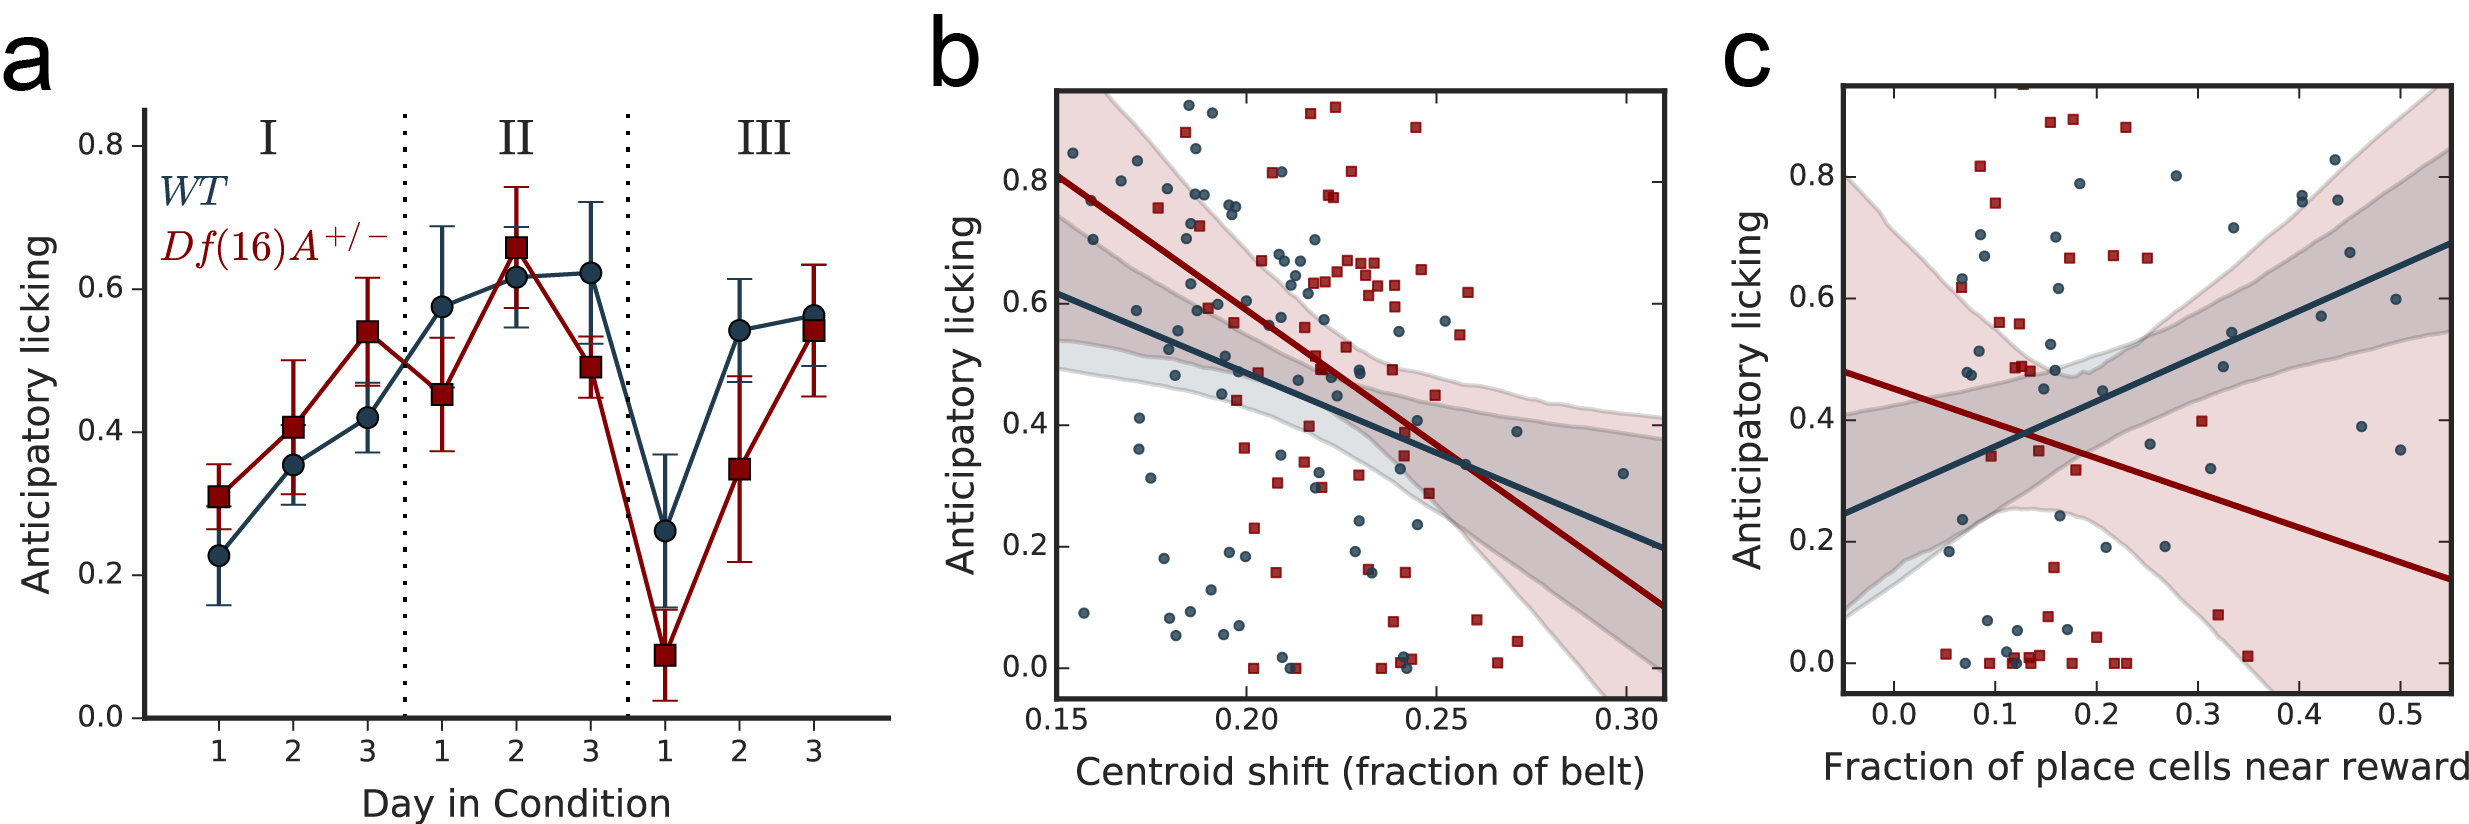
\includegraphics[width=0.9\textwidth]{df/FigSX_anticipatory_licking}
	\caption{}
	\label{fig:conclusions:anticipatory_licking}
\end{figure}
% \todo{include nucleus acumbens/VTA}

Hippocampal area CA1 receives a direct project from the entorhinal cortex via the temporoammonic pathway, which could shape their activity in a task- and learning-dependent manner. Grid cells in the medial entorhinal cortex are thought to contribute to a cognitive map of space by providing a metric framework for direction and distance \citep{Hafting2005}\citep{Jeffery2015a} and these cells directly project to hippocampal area CA1 \citep{Zhang2013}, though the nature of their influence on CA1 place cell activity is currently debated \citep{Wills2010}\citep{Langston2010}\citep{Koenig2011}\citep{Brandon2011a}. Recent studies \citep{Krupic2015a}\citep{Stensola2015a} have found evidence for warping of grid spacing to salient anchors points (walls), so it is tempting to speculate about a similar warp of grid cell spacing by the learned reward position.
While we did not record from area CA3 cells in the current study, previous studies \citep{Dupret2010a} have shown similar goal-directed remapping in CA1, but no remapping in CA3, leading to the possibility that area CA1 place cell activity is driven by stable CA3 representations and updated with environmental sensory input (border cells) and self-motion cues (grid cells) from the entorhinal cortex \citep{Bush2014a}.
Particularly, an increasing gradient of grid spacing centered about the reward would provide the perception of slower movement, thus delaying the firing of cells tuned to distance from boundaries and shifting all place cells towards the reward. The nature of border cells in a one-dimensional head-fixed environment is not entirely obvious, though there are salient belt fabric transitions that could similarly anchor a cognitive reference frame.
This interpretation predicts that after reward learning, a given grid module will have an increased scale, with spacing maximal farthest away from the reward (largest shift) and smallest near the reward (smallest shift).
Also, under conditions of grid cell map warping, we would expect a correlation between the local density of grid fields and the density of place cells.
By recording either grid cells directly from the medial entorhinal cortex or grid cell axons that project to CA1, we could directly test these predictions.

\todo[inline, color=yellow]{CA1 as source of enrichment, INs/neuromodulatory}
% Alternatively, CA1 could itself be the source of enrichment if 

\subsection{Long term stability in place cell population}
One of my first experiments with the \df/ mouse was to look at the long-term stability of CA1 spatial maps in a similar manner as \citeauthor{Ziv2013}.
Mice were trained to run head-fixed on our same cue-rich multi-fabric belts as I used in the \ac{GOL} task, but only for 1 session each day and the water reward was presented non-operantly once per lap at the same location every day.
I recorded CA1 pyramidal cell activity for at least 6 days without changing any aspects of the task.
By looking at the stability between spatial maps at progressively longer elapsed intervals I found that while the wildtype stability decreased from 1 day elapsed to 5 days elapsed, the \df/ spatial maps were surprisingly rigid for the entire 6 days (\autoref{fig:conclusions:chronic_stability}).

\begin{figure}
	\centering
	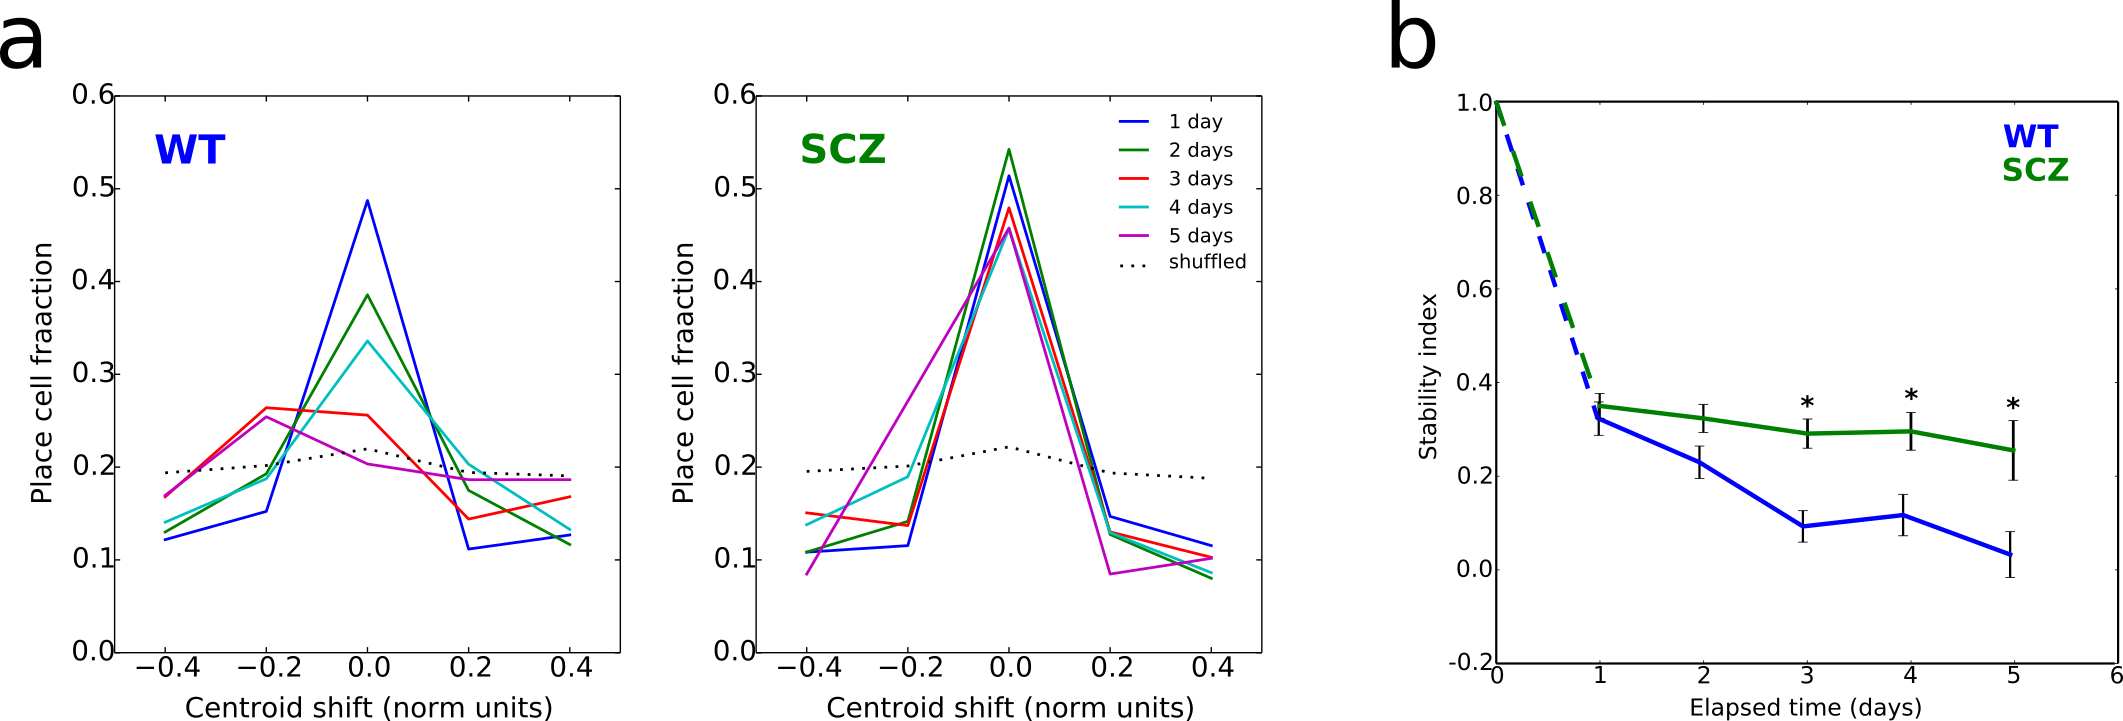
\includegraphics[width=0.9\textwidth]{df/chronic_stability}
	\caption{}
	\label{fig:conclusions:chronic_stability}
\end{figure}

\citeauthor{Ziv2013} actually found the wildtype mice to be more stable than what I observed, but I think this can be contributed to differences in task protocol.
In their task, mice were running in an already familiar environment, so the stability observed was reflective of an already stabilized spatial map.
In contrast, in our task the belt that conveys all of the spatial information was novel on day~1, therefore we observed the normal stabilization that occurs over the first few days of exposure to a novel environment.
This interpretation suggests that the \df/ mice immediately stabilize their spatial maps so that they don't allow for the normal stabilization process to occur.

This data needs further follow-up to completely interpret the results.
There was really no spatial learning in this version of the task.
Mice received water as long as they continued to run, it was delivered automatically every lap, and they didn't need to remember where that location was.
The first experiment I would run would be to change the reward schedule to require learning and memory.
Instead of a non-operant reward every lap, I would make it similar to the \ac{GOL} task; one rewarded zone where the water is only delivered if the mice actually lick there.
In this case I would expect to see several factors alternatively driving stability or rigidity.
First, wildtype mice showed a task-dependent stabilization from day-to-day, so we might see this effect over longer timescales as well.
Second, in Condition~III of my \ac{GOL} task I observed place cell enrichment of the reward location in the wildtpye mice, which could manifest as transient instability as cells remap to the reward, but then increased stability as they stabilize.
Finally, I observed neither of those effects in \df/ mice, so I don't necessarily expect this change to affect the stability of the \df/ place fields.

In addition, to see if the decreased stability in the wildtype mice relative to \citeauthor{Ziv2013} is truly due to environment novelty, we could either over-train the mice on the same belt on which we will eventually record place cell activity, or extend the protocol to 10 or more days so that we can alternatively discard the first few days and look at long-term stability relative to day 3 or 4.
I would expect to see increased stability in the wildtype mice, back to the level observed initially in the \df/ mice.
Assuming that both of these proposed manipulations increase stability in the wildtype mice, but don't affect the already increased \df/ stability, this would confirm an aberrantly fast place map rigidity in novel environments, and would suggest deficient novelty signaling in the \df/ mice, which may be linked to aberrant neuromodulatory signaling of novelty or generally with the proposed role of CA1 in novelty detection \citep{Li2003d}\citep{Barry2012c}\citep{Larkin2014}\citep{Nitz2004}.

\begin{figure}
	\centering
	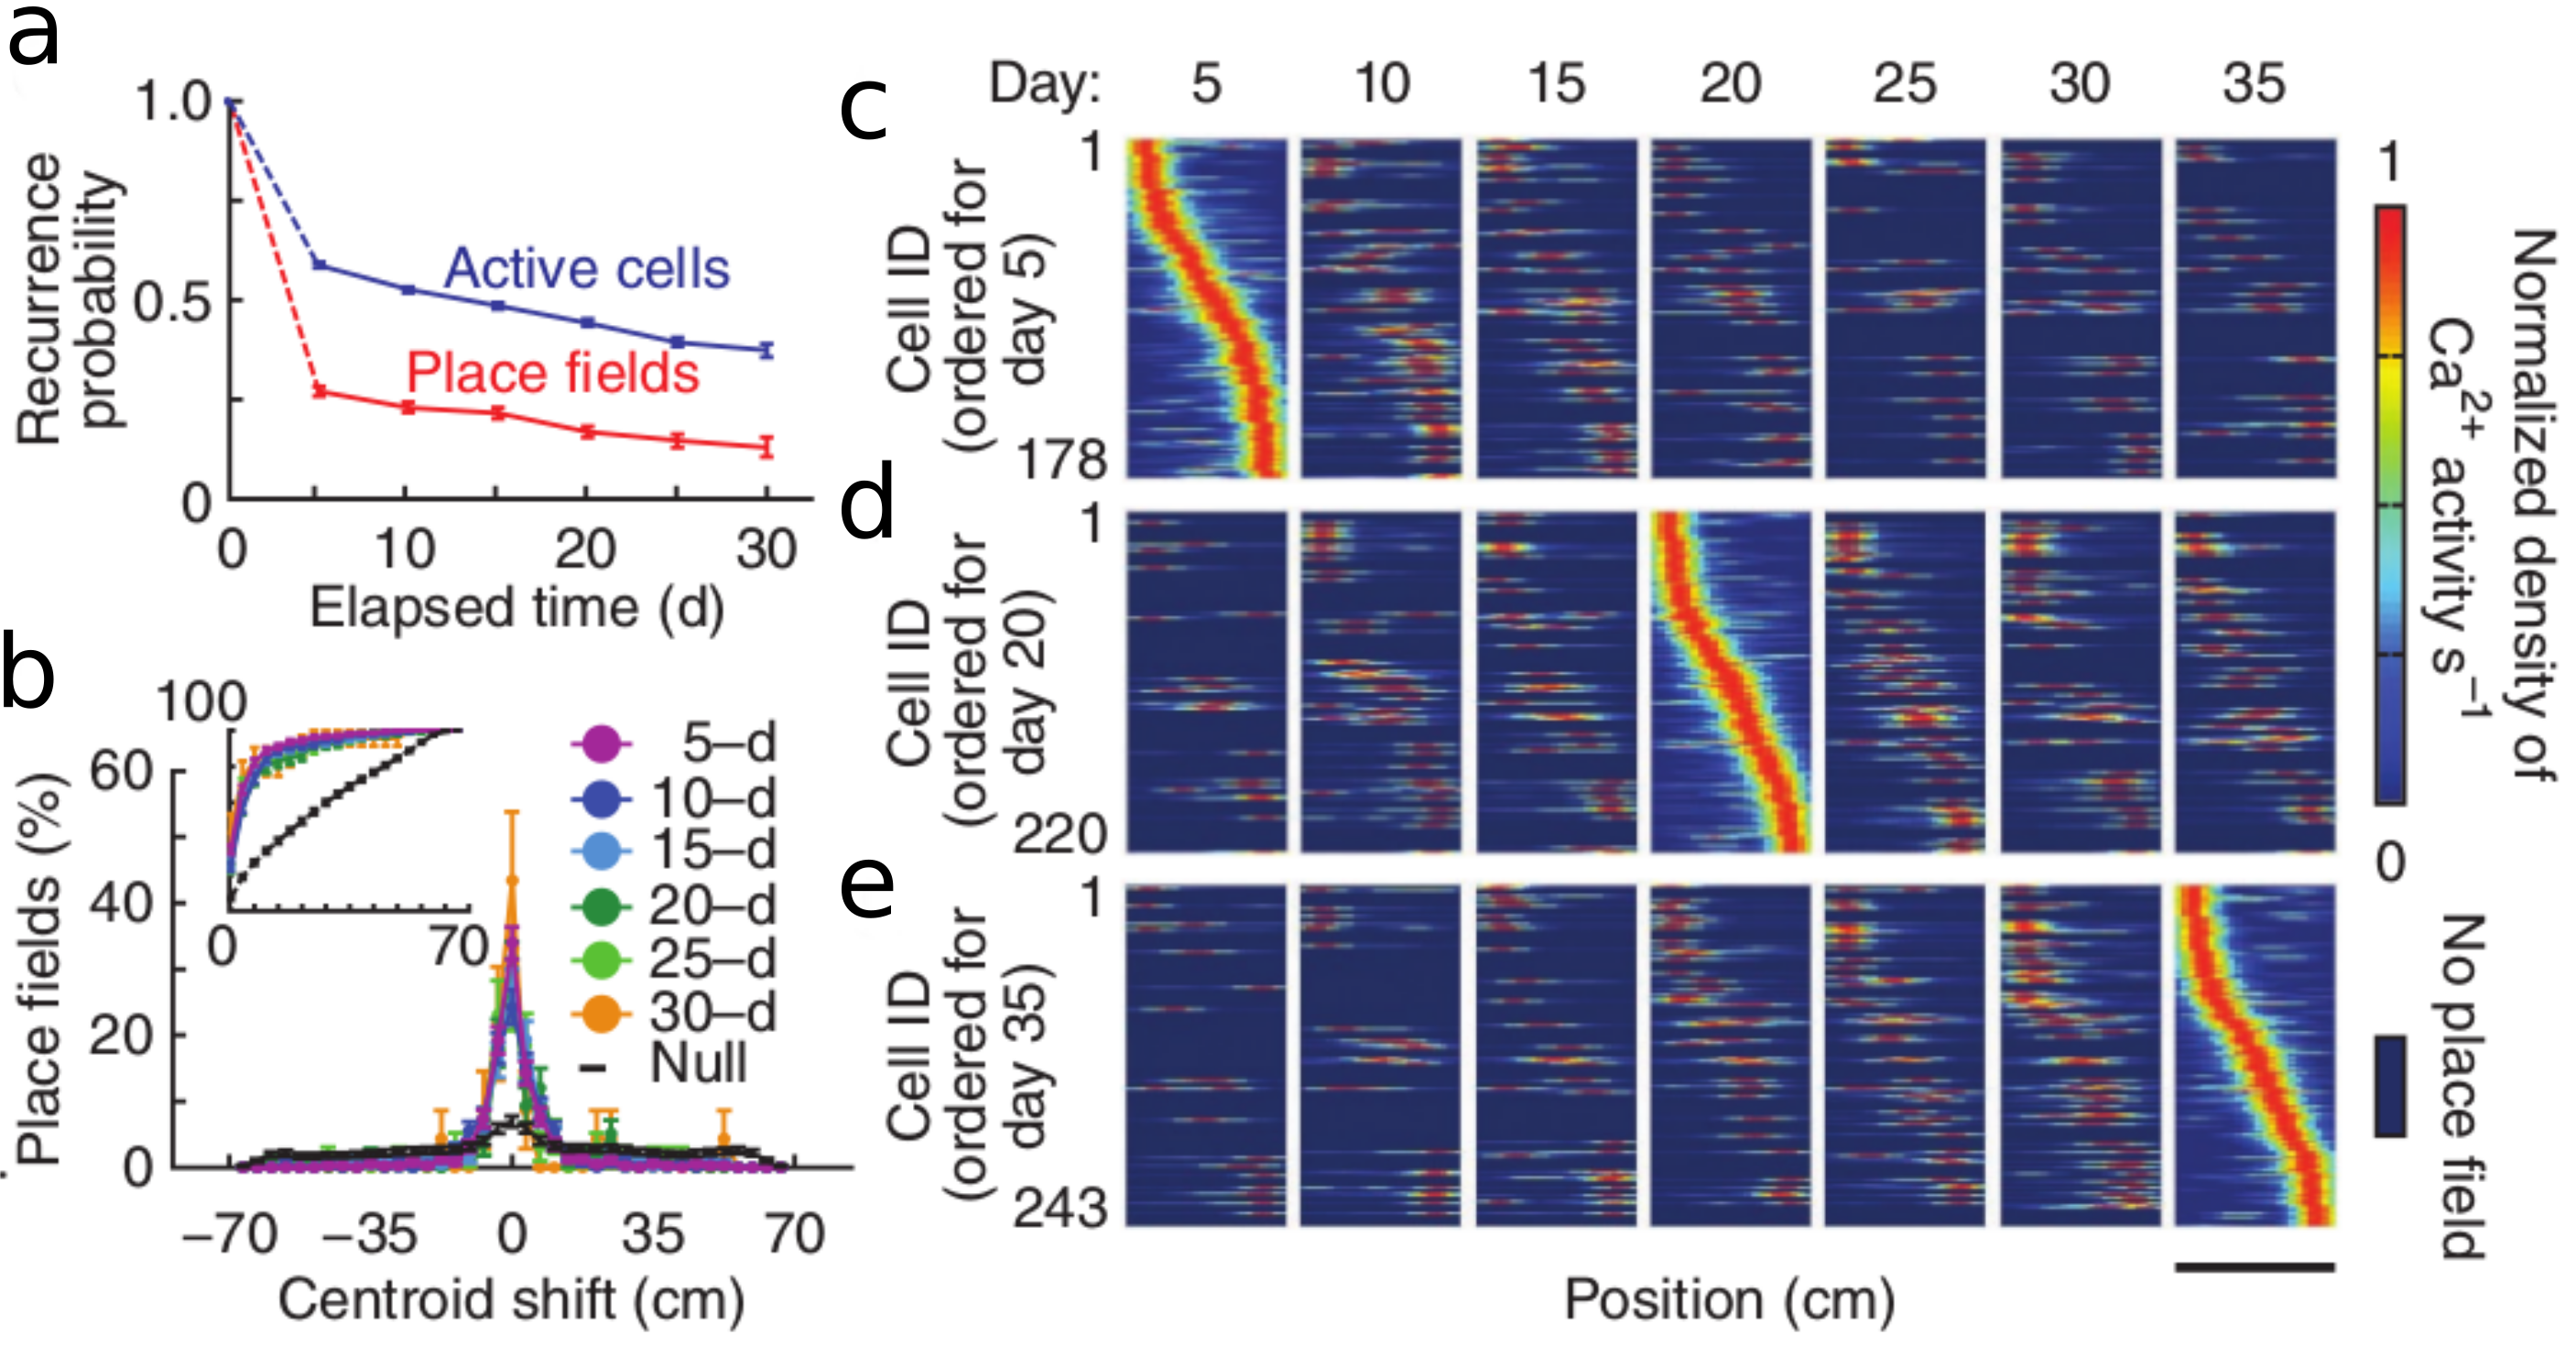
\includegraphics[width=0.75\textwidth]{intro/Ziv2013_stability_edit}
	\caption[Place field stability in Ziv et al.]{Place fields are spatially invariant and temporally stochastic while preserving a stable representation at the ensemble level.
	(a) If a cell had Ca\super{2+} activity in one session, the odds (blue data) that it also did in a subsequent session declined with time. If a cell had a statistically significant place field in one session, the odds (red data) that it had a place field in a subsequent session also declined with time. Mean~$\pm$~s.e.m.
	(b) Distributions of centroid shifts (colored by days between sessions, mean~$\pm$~s.e.m.) were indistinguishable (Kolmogorov-Smirnov test, P~$\geq$~0.17), sharply peaked at zero and highly distinct from the null hypothesis that place fields would randomly relocate (P~=~$4\times10^{-67}$, Kolmogorov-Smirnov test). Inset, cumulative histograms of shift magnitudes; 74-83\% were $\leq$7~cm. Median shift (3.5~cm) was much less than the median place field width (24~cm).
	(c-e) Place-field maps for cells found on multiple days, ordered by place fields' centroid positions on day~5 (c), day~20 (d) or day~35 (e). Data pooled across four mice.
	Reproduced from \citet{Ziv2013}.}
	\label{fig:conclusions:ziv_stability}
\end{figure}

\subsection{Neuromodulators in the \ac{HPC} of \df/ mice}
Place cell stability can be affected by salience, novelty, and attention, which has been shown to act through neuromodulatory inputs, including dopamine and acetylcholine.
In addition both dopamine and acetylchline have been implicated in \scz/ disease progression.
To search for aberrant salience/novelty/atention signaling in the \df/ mice I could directly image the activity of the dopaminergic and cholinergic axons projecting from the ventral tegmental area and medial septum, respectively, to area CA1 of the \ac{HPC}.
% and then use a combination of pharmacological, optogenetic and pharmacogenetic manipulations of each network component in order to dissect out the underlying circuit mechanisms of spatial memory deficits in the SCZ mutant mice.

Both principal neurons and local GABAergic interneurons are targeted by afferents from neuromodulatory nuclei, including cholinergic and GABAergic projections from the medial septum (MS) \citep{Klausberger2008}, serotonergic and glutamatergic projections from the raphe nuclei \citep{Varga2009}, dopaminergic projections from the ventral tegmental area (VTA) \citep{Gasbarri1997} and noradrenergic projections from the locus coeruleus \citep{Foote1983}.
Of these neuromodulatory projections, the dopaminergic-VTA and cholinergic-MS projections are of particular interest, since there is already extensive literature relating dopamine to \scz/ \citep{Davis1991} and the cholinergic projection is involved in normal hippocampal learning and memory \citep{Parent2004}.
Despite these well-characterized features of hippocampal neuromodulation, it remains unknown how the function of these circuits are altered in \scz/ during hippocampal-dependent behaviors.
